% LTeX: language=it

\section{Onde elettromagnetiche}

\begin{figure}[H]
    \centering

    % https://tikz.net/electromagnetic_wave/
    % Electromagnetic wave - colored
    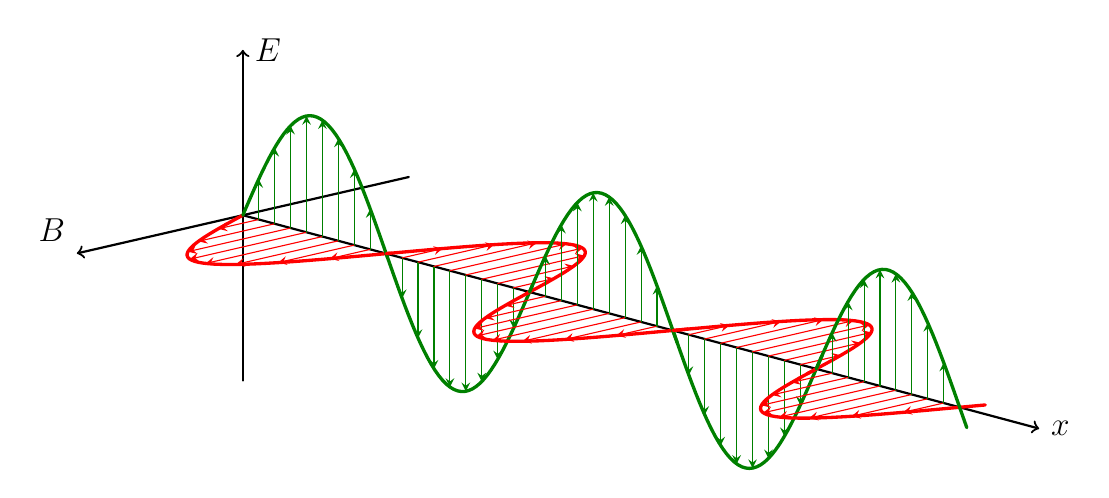
\begin{tikzpicture}[x=(-15:1.2), y=(90:1.0), z=(-150:1.0),
            line cap=round, line join=round,
            axis/.style={black, thick,->},
            vector/.style={>=stealth,->}]
        \large
        \def\A{1.5}
        \def\nNodes{5} % use even number
        \def\nVectorsPerNode{8}
        \def\N{\nNodes*40}
        \def\xmax{\nNodes*pi/2*1.01}
        \pgfmathsetmacro\nVectors{(\nVectorsPerNode+1)*\nNodes}

        \def\drawENode{ % draw E node and vectors with some offset
            \draw[Green,very thick,variable=\t,domain=\iOffset*pi/2:(\iOffset+1)*pi/2*1.01,samples=40]
            plot (\t,{\A*sin(\t*360/pi)},0);
            \foreach \k [evaluate={\t=\k*pi/2/(\nVectorsPerNode+1);
                        \angle=\k*90/(\nVectorsPerNode+1);}]
            in {1,...,\nVectorsPerNode}{
                    \draw[vector,Green]  (\iOffset*pi/2+\t,0,0) -- ++(0,{\A*sin(2*\angle+\iOffset*180)},0);
                }
        }
        \def\drawBNode{ % draw B node and vectors with some offset
            \draw[Red,very thick,variable=\t,domain=\iOffset*pi/2:(\iOffset+1)*pi/2*1.01,samples=40]
            plot (\t,0,{\A*sin(\t*360/pi)});
            \foreach \k [evaluate={\t=\k*pi/2/(\nVectorsPerNode+1);
                        \angle=\k*90/(\nVectorsPerNode+1);}]
            in {1,...,\nVectorsPerNode}{
                    \draw[vector,Red]  (\iOffset*pi/2+\t,0,0) -- ++(0,0,{\A*sin(2*\angle+\iOffset*180)});
                }
        }

        % MAIN AXES
        \draw[axis] (0,0,0) -- ++(\xmax*1.1,0,0) node[right] {$x$};
        \draw[axis] (0,-\A*1.4,0) -- (0,\A*1.4,0) node[right] {$E$};
        \draw[axis] (0,0,-\A*1.4) -- (0,0,\A*1.4) node[above left] {$B$};

        % draw (anti-)nodes
        \foreach \iNode [evaluate={\iOffset=\iNode-1;}] in {1,...,\nNodes}{
                \ifodd\iNode \drawBNode \drawENode % E overlaps B
                \else        \drawENode \drawBNode % B overlaps E
                \fi
            }

    \end{tikzpicture}
    \caption{Onda elettromagnetica}
\end{figure}


